% This is part of Un soupçon de mathématique sans être agressif pour autant
% Copyright (c) 2012
%   Laurent Claessens
% See the file fdl-1.3.txt for copying conditions.

\chapter{Statistiques descriptives}

%+++++++++++++++++++++++++++++++++++++++++++++++++++++++++++++++++++++++++++++++++++++++++++++++++++++++++++++++++++++++++++
\section{Activité : mois de naissance}
%+++++++++++++++++++++++++++++++++++++++++++++++++++++++++++++++++++++++++++++++++++++++++++++++++++++++++++++++++++++++++++

Prendre les mois de naissance des élèves, en séparant les groupes.
\begin{enumerate}
    \item
        Quel groupe a la proportion de naissance en mars la plus grande ?
    \item
        En tout quelle est la proportion des naissances en avril ?
    \item 
        Est-ce qu'on peut voir l'effet comme quoi les mois de \( 31\) jours son plus longs ? 
        \begin{enumerate}
            \item
                Quelle est la proportion d'élèves nés dans un mois de \( 31\) jours ?
            \item
                Il y a \( 7\) mois de $31$ jours contre \( 5\) de moins. Donc le résultat est biaisé.
            \item
                Calculer la \emph{fréquence} des naissances en naissances par mois.
        \end{enumerate}
\end{enumerate}

%+++++++++++++++++++++++++++++++++++++++++++++++++++++++++++++++++++++++++++++++++++++++++++++++++++++++++++++++++++++++++++
\section{Regardons des graphiques}
%+++++++++++++++++++++++++++++++++++++++++++++++++++++++++++++++++++++++++++++++++++++++++++++++++++++++++++++++++++++++++++

Les graphiques sont souvent tirés de wikipédia. Si vous voulez plus d'informations, lisez \url{http://www.manicore.com/}, ou bien regardez le cours \href{http://www.mines-paristech.fr/ingenieurcivil/SitesIC/Balado/Climat_som.html}{en ligne}, en particulier la deuxième heure du troisième cours donne les facteurs d'émissions dans le monde et en France.

%---------------------------------------------------------------------------------------------------------------------------
\subsection{Émissions par secteurs}
%---------------------------------------------------------------------------------------------------------------------------

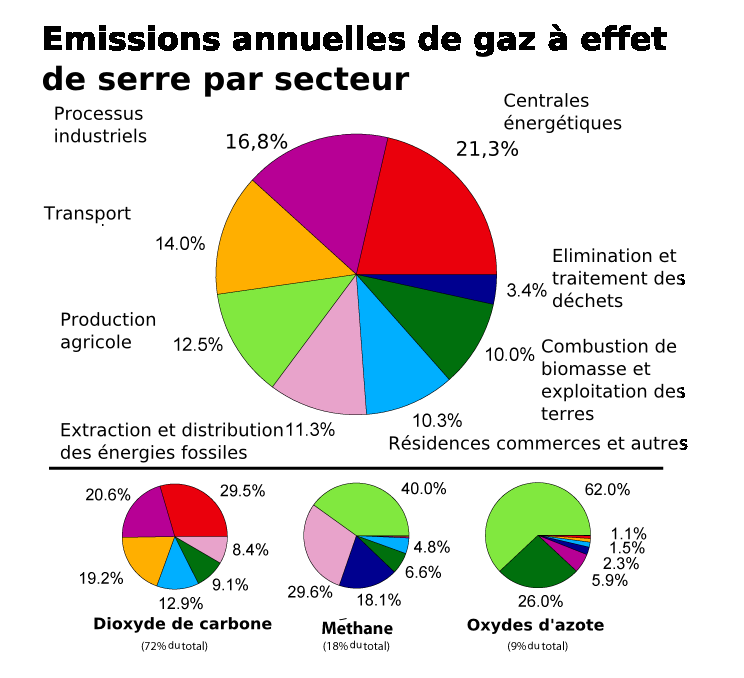
\includegraphics[width=17cm]{Emission_de_GES.png}
Graphique en provenance de l'article \wikipedia{fr}{Gaz_à_effet_de_serre}{gaz à effet de serre} de wikipédia.

\begin{enumerate}
    \item
        Quel est le secteur qui émets le plus ?
    \item
        Est-ce que l'agriculture émet beaucoup de dioxyde de carbone ?
    \item
        À partir des deux graphiques du bas, est-ce que vous êtes capables de retrouver le \( 12.5\%\) de l'agriculture donnés dans le graphique du haut ?
\end{enumerate}

%---------------------------------------------------------------------------------------------------------------------------
\subsection{Découvertes de pétrole}
%---------------------------------------------------------------------------------------------------------------------------

Regardons un instant le graphique suivant, provenant de l'article \wikipedia{fr}{Pic_pétrolier}{Pic pétrolier} de wikipédia.

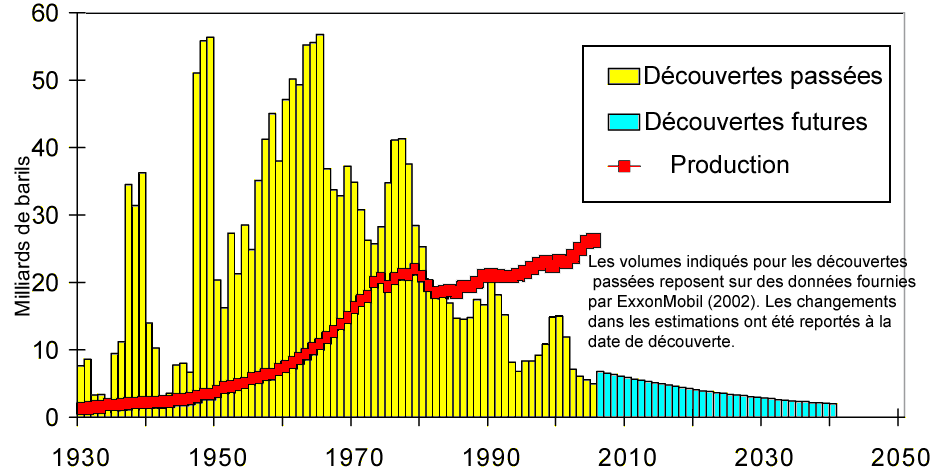
\includegraphics[width=17cm]{Decouvertes-petrole.png}

\begin{enumerate}
    \item
        Quelle est l'année où on a découvert le plus de pétrole ?
    \item
        Quelle est l'année où on a consommé le plus de pétrole ?
    \item
        En quelles années on a consommé autant qu'on a découvert ?
    \item
        Que pensez-vous de l'affirmation «ce qui reste comme réserve est la surface jaune au-dessus de la ligne rouge» ?
\end{enumerate}
Pour aller plus loin, remarquer la cassure assez nette de la croissance de la production vers 1975. Juste par curiosité, faites quelque recherches sur l'histoire de la croissance économique, de la dette publique et le chômage en France (et en Europe). Est-ce que les années 1970 ont été spéciales de ce point de vue ?

%---------------------------------------------------------------------------------------------------------------------------
\subsection{Températures}
%---------------------------------------------------------------------------------------------------------------------------

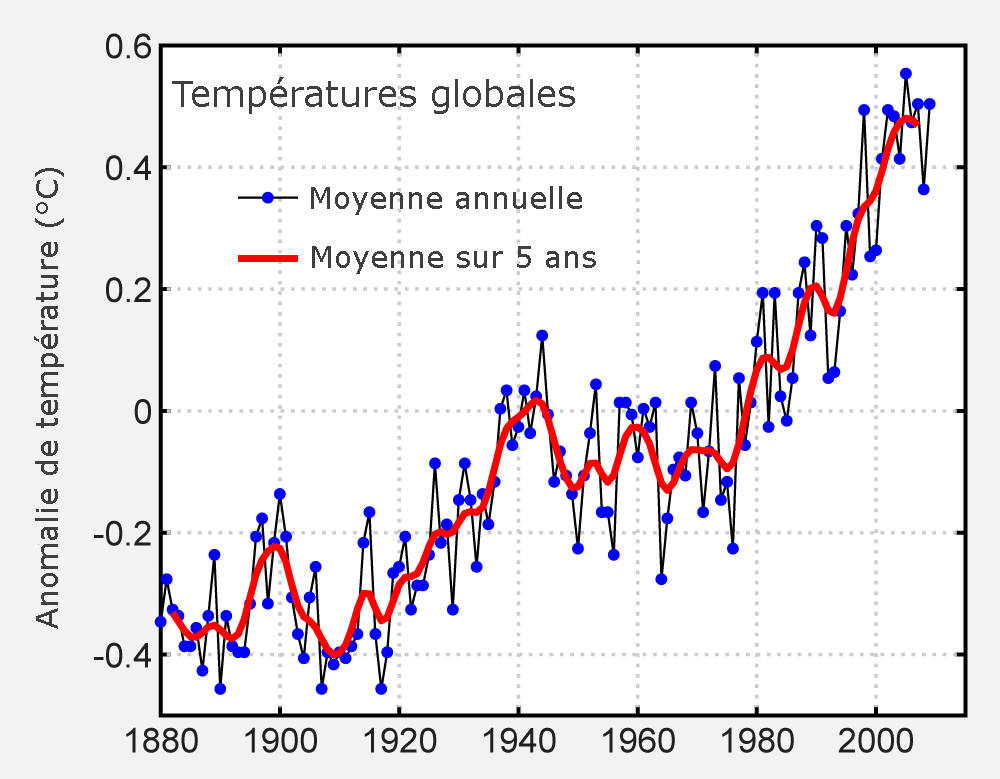
\includegraphics[width=17cm]{Instrumental_Temperature_Record_fr.png}
Graphique en provenance de l'article \wikipedia{fr}{Réchauffement_climatique}{réchauffement climatique} de wikipédia.

Le zéro de ce graphique est la moyenne 1961-1990.

\begin{enumerate}
    \item
        Quelle est la dernière année «normale» ?
    \item
        Quelle est l'année la plus chaude ?
    \item
        Quelle est l'année la plus froide ?
\end{enumerate}

%---------------------------------------------------------------------------------------------------------------------------
\subsection{Consommation de pétrole}
%---------------------------------------------------------------------------------------------------------------------------

Lire le tableau suivant :
\begin{center}
\begin{tabular}[h]{|c|c|c|c|c|c|c|c|c|}
année&
2001&
2002&
2003&
2004&
2005&
2006&
2007&
2008\\
consommation (Mb/j)&
76,8&
77,7&
79,1&
81,8&
83,1&
83,8&
84,9&
84,5
\end{tabular}
\end{center}

Calculer le pourcentage d'augmentation année par année. Que s'est-il passé en 2008 ?

%---------------------------------------------------------------------------------------------------------------------------
\subsection{À faire fonctionner}
%---------------------------------------------------------------------------------------------------------------------------

Les graphiques montrent
\begin{enumerate}
    \item

        À la figure \ref{LabelFigautomaticDSpcb}, \( y=\) proportion des étudiants ayant obtenu plus que \( x\)
    \item
        À la figure \ref{LabelFigautomaticDSpbt}, \( y=\) moyenne des étudiants ayant obtenu plus que \( x\). Par construction, le tout premier point de ce graphique est la moyenne de tout le groupe.
    \item
        À la figure \ref{LabelFigautomaticDSavb}, \( y=\) proportion des étudiants ayant obtenu dans \( \mathopen[ x-0.5 , x+0.5 \mathclose]\).
\end{enumerate}

\newcommand{\CaptionFigautomaticDSpcb}{Moyenne des étudiants ayant obtenus plus que \( x\)}
\input{Fig_automaticDSpcb.pstricks}

\newcommand{\CaptionFigautomaticDSpbt}{Proportion des étudiants ayant obtenus plus que \( x\)}
\input{Fig_automaticDSpbt.pstricks}

\newcommand{\CaptionFigautomaticDSavb}{proportion des étudiants ayant obtenu dans \( x\pm 0.5\)}
\input{Fig_automaticDSavb.pstricks}

%+++++++++++++++++++++++++++++++++++++++++++++++++++++++++++++++++++++++++++++++++++++++++++++++++++++++++++++++++++++++++++
\section{Théorie}
%+++++++++++++++++++++++++++++++++++++++++++++++++++++++++++++++++++++++++++++++++++++++++++++++++++++++++++++++++++++++++++

\begin{definition}
    Une \defe{population}{population} est un ensemble fini. Une \defe{série statistique}{série statistique} sur une population est une fonction qui à chaque élément (individu) de la population fait correspondre une valeur.

    L'\defe{effectif}{effectif} d'une valeur est le nombre d'individus correspondant à la valeur.

    La \defe{fréquence}{fréquence} d'une valeur est le rapport
    \begin{equation}
        f=\frac{ \text{effectif de la valeur} }{ \text{effectif total} }
    \end{equation}
    où par «effectif total» nous entendons la taille de la population totale.
\end{definition}



%+++++++++++++++++++++++++++++++++++++++++++++++++++++++++++++++++++++++++++++++++++++++++++++++++++++++++++++++++++++++++++
\section{Repères, distances, milieu}
%+++++++++++++++++++++++++++++++++++++++++++++++++++++++++++++++++++++++++++++++++++++++++++++++++++++++++++++++++++++++++++

%---------------------------------------------------------------------------------------------------------------------------
\subsection{Activité}
%---------------------------------------------------------------------------------------------------------------------------

Si nous plaçons un point sur le tableau, comment faire pour mettre un point au même endroit sur le tableau de la classe d'à côté ?

%---------------------------------------------------------------------------------------------------------------------------
\subsection{Repère}
%---------------------------------------------------------------------------------------------------------------------------

\begin{definition}
    Un \defe{repère orthonormé}{repère!orthonormé} du plan est la donné de trois points \( O\), \( I\), \( J\) formant un triangle rectangle isocèle en  \( O\).
\end{definition}
<++>

%---------------------------------------------------------------------------------------------------------------------------
\subsection{Exercices}
%---------------------------------------------------------------------------------------------------------------------------

\Exo{Seconde-0001}
\Exo{Seconde-0002}
\Exo{Seconde-0003}
\Exo{Seconde-0004}
\Exo{Seconde-0005}
\Exo{Seconde-0006}
\Exo{Seconde-0007}
\Exo{Seconde-0008}
\Exo{Seconde-0009}
\Exo{Seconde-0010}
\Exo{Seconde-0011}
\Exo{Seconde-0012}
\Exo{Seconde-0013}
\Exo{Seconde-0021}

%+++++++++++++++++++++++++++++++++++++++++++++++++++++++++++++++++++++++++++++++++++++++++++++++++++++++++++++++++++++++++++
\section{Petits exercices de calcul mental}
%+++++++++++++++++++++++++++++++++++++++++++++++++++++++++++++++++++++++++++++++++++++++++++++++++++++++++++++++++++++++++++

\Exo{Seconde-0014}
\Exo{Seconde-0015}
\Exo{Seconde-0016}
\Exo{Seconde-0017}
\Exo{Seconde-0018}
\Exo{Seconde-0019}
\Exo{Seconde-0020}
